\chapter{Realizzazione e Testing}
\label{chap:realizzazione-testing}

\section{Realizzazione delle componenti}
\subsection{Componenti}

\subsection{Versionamento del codice}

\subsection{Documentazione}
L'implementazione della libreria prodotta è stata documentata tramite l'utilizzo di \textit{Confluence}, la piattaforma
di gestione della conoscenza e di collaborazione sviluppata da \textit{Atlassian}. \newline
La documentazione, su richiesta dell'azienda, è stata redatta in lingua inglese, attraverso una descrizione dettagliata
delle componenti e delle funzionalità offerte dalla libreria. \newline

\begin{figure}[H]
    \centering
    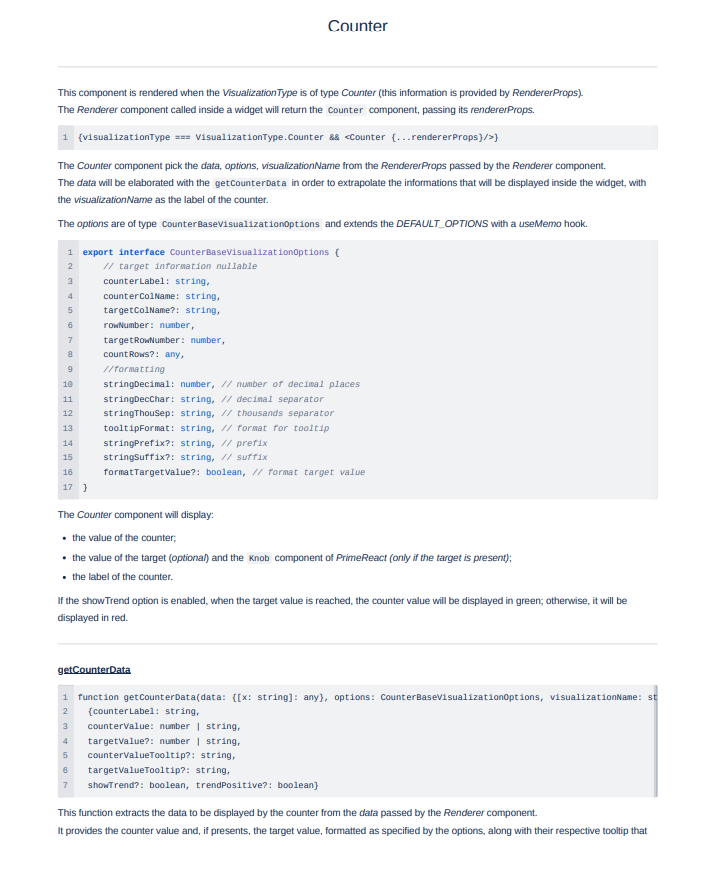
\includegraphics[alt={Esempio documentazione Confluence}, width=1 \textwidth]{img/ex_confluence.png}
    \caption{Esempio documentazione Confluence}
    \label{fig:ex_confluence}
\end{figure}

La documentazione è stata strutturata in modo da essere facilmente consultabile e comprensibile, con l'obiettivo di
fornire un supporto efficace agli sviluppatori futuri che potrebbero dover utilizzare la libreria. \newline
La produzione di una buona documentazione ricopre infatti un ruolo fondamentale al fine di garantire la manutenibilità
del codice e la facilità di comprensione delle funzionalità offerte dalla libreria, in modo da ridurre i tempi di
apprendimento e di sviluppo necessari per gli utilizzi futuri del prodotto implementato.

\section{Testing}
